In this Section we describe the methodology that we have followed to deploy a Hadoop cluster instance inside the FedCloud federated cloud infrastructure. 
%Basically, it consists of two processes: 
%\begin{enumerate}
%\item \emph{Cluster startup}: obtaining the resources necessary to form the cluster from each of the sites in FedCloud and configure the Hadoop cluster
%\item \emph{Benchmarks}: loading the data sets and running various MapReduce jobs
%\end{enumerate}
%Each of these processes is described in more detail in the following subsections.

\subsection{Cluster startup}
\label{ssect-cluster}
% Hadoop configuration
%% Hadoop 1.0.3
%% Oracle Java JDK 1.6.0_33
%% Modules

% Basics about Hadoop services needed: hadoop-master, slaves
The Hadoop clusters consists of one \emph{master} node and a variable number of \emph{slave} nodes depending on the size of the cluster. For example in the case of a 101 node cluster, one node will be configured as master and the remaining 100 as slaves. The master node will run the \emph{namenode}, \emph{secondarynamenode} and \emph{jobtracker} services and each of the slaves will run just the \emph{tasktracker} and \emph{datanode} services.

%% VM template & Marketplace

%A general overview of the overall cluster startup process is given in Figure~\ref{fig:client}.

%A customized virtual machine (VM) image template that includes all the software necessary was created. This image is based on Scientific Linux 6.4 and contains the following customizations:
%\begin{itemize}
%\item \emph{Firewall:} only inter-cluster communication allowed except for remote ssh access.
%\item \emph{SSH:} ssh key only authentication.
%\item \emph{Java:} both Oracle Java JDK 1.6 and 1.7 are included.
%\item \emph{Hadoop:} different versions of Hadoop are included up to 1.2.1 (latest stable version in the v1 branch). The configuration using Modules makes easy to include additional versions and decide the one we want to use when starting the Hadoop cluster.
%\item \emph{Modules:} allow the user to select different Hadoop environments.
%\end{itemize}

A customized virtual machine (VM) image was created including different versions of Hadoop (up to 1.2.1) and Oracle Java JDK (both 1.6 and 1.7).
This customized image was registered in the EGI Marketplace~\cite{marketplace} which provides a common place where where we can can store images. The Marketplace does not store the VM images into a common repository, it just shows which resource providers (RPs) have the VM image available at their endpoint. This means that each RP has to manually download the image to his local site in order to make it available at his endpoint. 

% Client: rOCCI + VOMS
To instantiate the virtual machines that will form the Hadoop cluster we used rOCCI~\cite{rocci}, the implementation of the OCCI 1.1 specification developed by one of the authors, using VOMS proxy credentials. The new rOCCI implementation provides several advantages like the fact that we are able to avoid the previous issue that all user certificates request are mapped to a single ONE\_USER account.
Additionally, the usage of VOMS over plain X509 auth greatly simplifies the access to the different sites that form FedCloud without the need to request each site to give access to our X509 certificate's DN.

FedCloud does not count with a workload management system, so each VM creation request must be sent to the appropriate endpoint, and we should take care of partitioning the cluster between the different FedCloud resource providers.

%\begin{figure}[h]
%\centering
%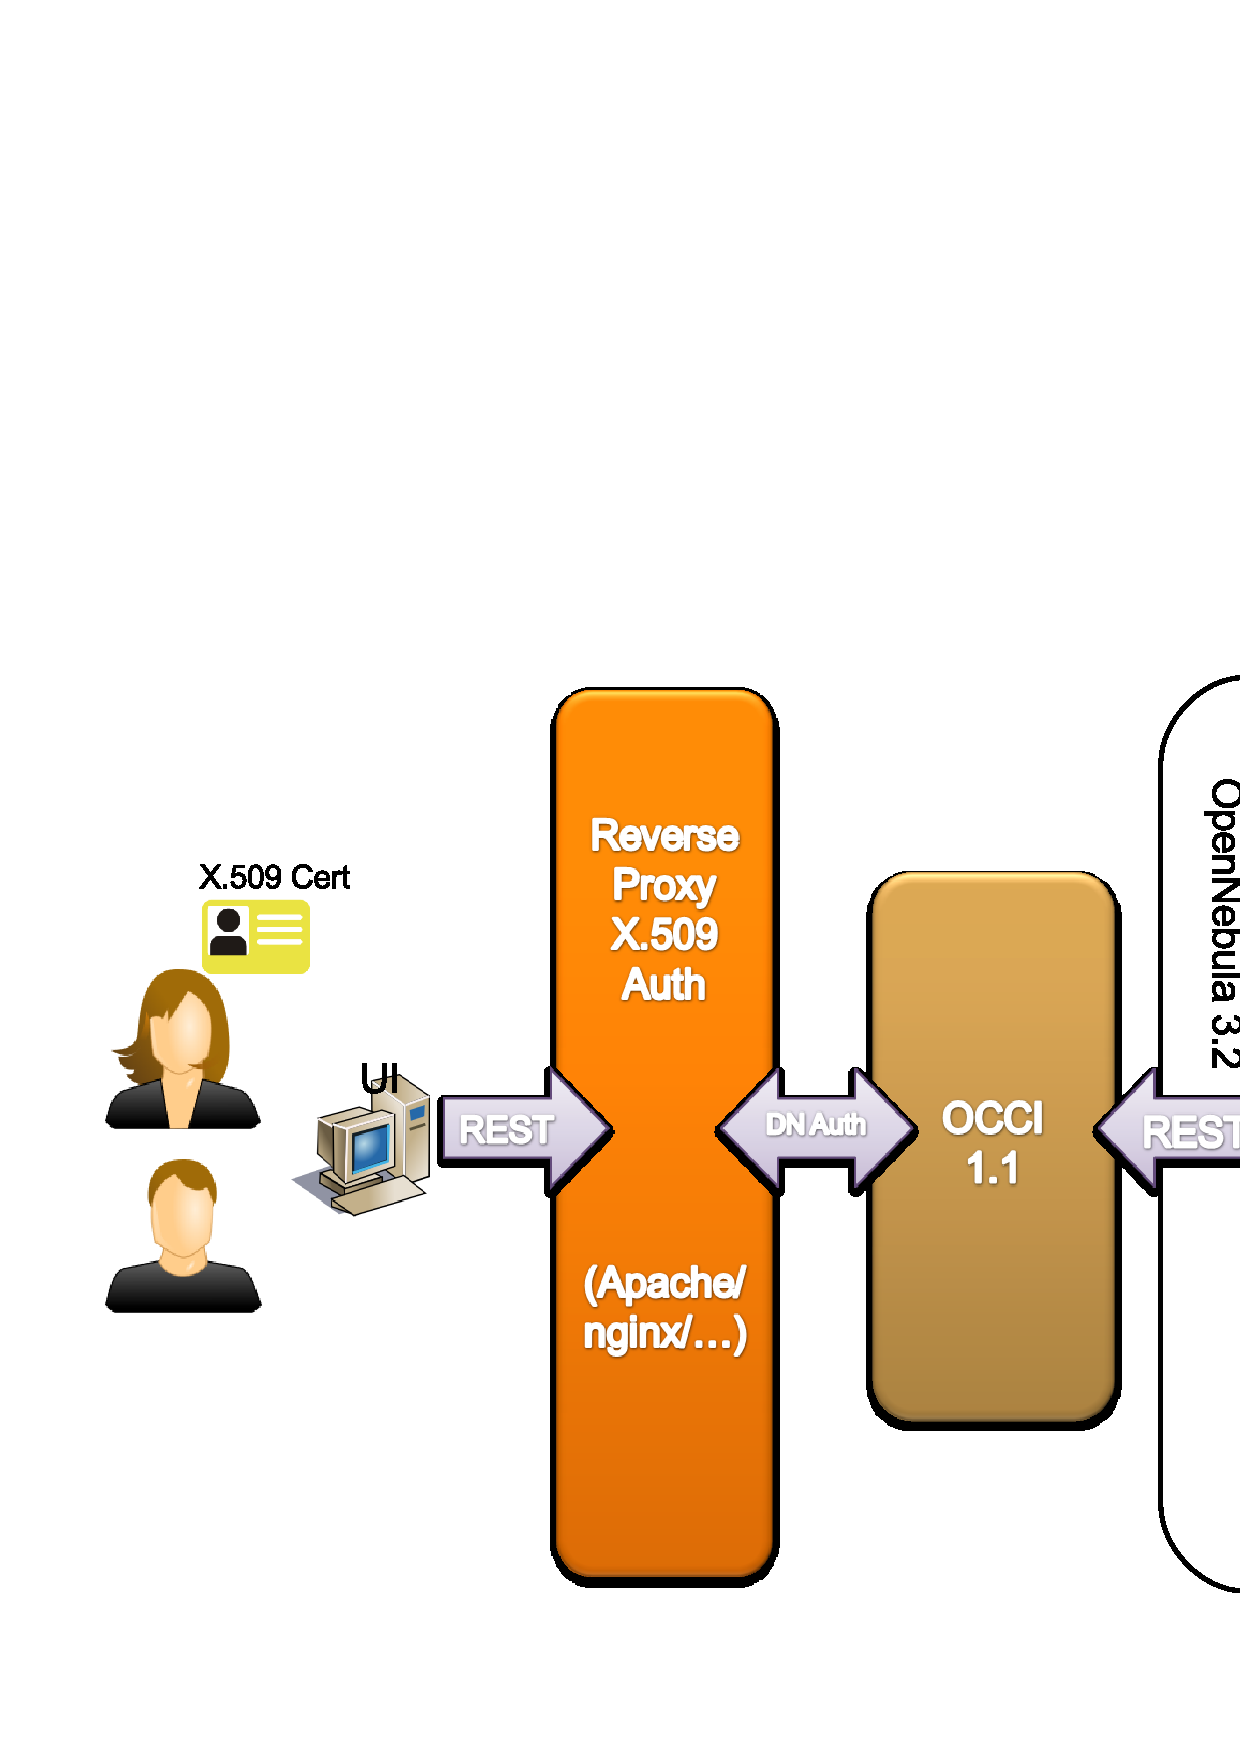
\includegraphics[width=0.8\textwidth]{figures/occi_opennebula.png}
%\caption{OCCI 1.1 server and x509 auth for OpenNebula.}
%\label{fig:occi1}
%\end{figure}

%\begin{figure}[h]
%\centering
%\includegraphics[width=\textwidth]{figures/client-v2.png}
%\caption{Cluster startup process using rOCCI and VOMS from a single UI.}
%\label{fig:client}
%\end{figure}

% Resources used
In order to increase the concurrent number of VMs, we used small size VM instances with 1GB of RAM and 1 CPU for the small and medium-size use cases and 2GB of RAM and 1 core for the TeraGen and TeraSort bechmarks.


% Tuned configuration 
The tuned configuration parameters for running the selected use cases are given in Table \ref{table:conf}. The column type identifies the configuration file where the parameter is set, the complete configuration files can be found at~\cite{scripts}.

These parameters have been selected to tune the Hadoop cluster to the resources available (1GB of RAM and 1 CPU per node). The $dfs.replication$ parameter indicates how many copies we want to store of each block, in this case we use three replicas that will allow different nodes to execute the same MapReduce tasks--speculative execution--mitigating the performance degradation that could be experienced in a heterogeneous cluster with VMs running under hypervisors with different load conditions. The $mapred.tasktracker.map.tasks.maximum$ and $reduce.tasks.maximum$ are set to 1 because we only have 1 CPU available to run both services and the HADOOP\_HEAPSIZE is set to 512MB to allow both running at the same time without exhausting the node's memory. The number of reduce tasks, $mapred.reduce.tasks$, is set to 95\% of the number of slaves in the Hadoop cluster. 

Our Hadoop installation will cope with two very different use cases that influence our decission about the $dfs.block.size$ values to use. In the case of the Encyclop{\ae}dia Britannica's use case the block size is set to 1MB and in the Wikipedia's use case, that uses a much larger data set, to 64MB. Under these conditions both use cases generate less than 700 total MapReduce tasks which can be handled well by the Hadoop master node which has only 1GB of RAM and 1 CPU. For the TeraGen and TeraSort becnhmarks we use an even larger block size of 128MB.


%% table with the parameters used
% TODO: complete the table
\begin{table}[h!]
\caption{Tuned Hadoop configuration for small VM instances. It includes both the HDFS and MapReduce parameters used.}
\label{table:conf}
%
\vspace{-0.5em}
%
\begin{center}
\begin{tabular}{ccc}
\toprule
%Parameter				& Type\tablenotemark[a] & Value	 	\\
Parameter				& Type 			& Value	 	\\
\midrule
$fs.inmemory.size.mb$			& core-site		& 200MB	 	\\
$io.file.buffer.size$                  	& core-site		& 128KB  	\\
$mapreduce.task.io.sort.factor$ 	& core-site		& 100	 	\\
$mapreduce.task.io.sort.mb$ 	 	& core-site		& 100	 	\\
$mapred.tasktracker.map.tasks.maximum$ 	& mapred-site		& 1	 	\\
$mapred.tasktracker.reduce.tasks.maximum$ & mapred-site		& 1	 	\\
$mapred.reduce.tasks$ 			& mapred-site		& $0.95\times$\emph{num.~slaves} \\
$dfs.datanode.du.reserved$ 		& hdfs-site		& 1GB	 	\\
$dfs.block.size$ 			& hdfs-site		& 1MB / 64MB 	\\
$dfs.replication$ 			& hdfs-site		& 3	 	\\
HADOOP\_HEAPSIZE            	 	& hadoop-env   		& 512MB 	\\
%HADOOP\_OPTS                	 	& hadoop-env   		& $-XX:+UseParallelGC$ 	\\
%                             	 	&              		& $-Djava.net.preferIPv4Stack=true$ 	\\
%
%(1,5,0)		& 0.0645	& 0.0689\tablenotemark[d]	& $2 \times 10^{-4}$		\\
%
\bottomrule
\multicolumn{3}{c}{\rule{0.98\textwidth}{0em}}\\
%\rule{0.3\textwidth}{0cm} & \rule{0.2\textwidth}{0cm} &  \\
\end{tabular}
\end{center}
%\vspace{-3.5em}
%\tablenotetext[a] {Identifies the configuration file where the parameter is set, the complete configuration files can be found at \url{https://github.com/grid-admin/hadoop}}
\end{table}


%% TODO: Explain the values of the parameters used


\subsection{Benchmarks}
\label{ssect-execution}

In order to evaluate the suitability of FedCloud to perform Big Data analytics using Hadoop we selected the TeraGen and TeraSort benchmarks as well as two use cases representing usual small and medium-size jobs. These use cases use real data sets and a fairly common MapReduce operation.

% TeraGen/TeraSort
In the Big Data arena the TeraGen and TeraSort benchmarks could be considered the equivalent of Linpack in HPC. There is even a list equivalent to the well-know Top500 list of the most powerful supercomputers in the world. This list was created by Jim Gray and it is known as the Sort Benchmarks list~\cite{sortbenchmark}. This list is not restricted to Hadoop clusters, and any Big Data system that is able to sort files can compete to appear there. Currently the largest sort rate is achieved by a Hadoop cluster of 2100 nodes that reaches a sort rate of 1.42TB/min~\cite{sortbenchmarkyahoo}.

TeraGen is the part of the bechmark that generates the input data set that will be used by TeraSort. It can be configured to run in parallel using the whole cluster so the throughtput it obtains is much higher than a standard HDFS put operation.

TeraSort is a standard MapReduce sort job that uses a custom partitioner with a sorted list of $N-1$ sampled keys to guarantee that the output keys of reduce $n$ are lower than the output keys of reduce $n+1$. This allows the concatenation of all the output files generated by each Reducer to produce one ordered output file. 

% Selected use cases
The selected use cases using two well-known data sets which are quite representative of a broad range of jobs that could be performed in a Hadoop cluster--most MapReduce jobs are based on the same type of operations--. The use cases were run both in a federated cluster deployment and in a one-site-only cluster deployment, allowing us to compare the results and analyze the degradation when using remotely distributed resources.

% Encyclopaedia Britannica 1911: 176MB
%% -put (5 runs)
%%% Upload from hadoop-master
%% wordcount (5 runs)
The first use case, representing small-size Hadoop jobs, is based in the Encyclop{\ae}dia Britannica\cite{britannica} data set--the 1911 version that is already in the public domain--. This represents a rather small data set of just 176MB, so that this use case can be considered as a small scale benchmark that will serve to evaluate the expected degradation in performance due to fact that we will be using federated resources located at different sites. The data set is downloaded directly from the master node and later on it is distributed from there to the slaves, what is called a \emph{put} operation in Hadoop argon. This use case has a great overload due to the creation of rather small MapReduce tasks that will stress the communication system because it uses a rather small block size of just 1MB, so each map operation has little to process.

% Wikipedia: 41GB
%% -put (1 run)
%%% Upload from UI (hadoop-master does not have enough space to store it)
%% wordcount (5 runs)
The second use case, representing medium-size Hadoop jobs, is based in the Wikipedia\cite{wikipedia} data set. This represents a much larger data set comprising 41GB, so it can be considered a more realistic benchmark of a medium-size Hadoop job. Due to the size of the data set the files could not be downloaded directly in the master node so the \emph{put} operation is done directly from our local Hadoop client. This use case will incur in a lower task creation penalization because it uses a larger block size of 64MB, so each map task will take much longer than the time needed for its creation.

 
Both use cases were run for different cluster sizes ranging from 10 to 101. In all the executions we measured two parameters:
\begin{enumerate}
\item \emph{The put time:} the time to load the files into the Hadoop HDFS filesystem 
\item \emph{The wordcount time:} the time to perform a simple wordcount MapReduce job that computes the number of occurrences of each word over the complete data set. 
\end{enumerate}
All the measurements where repeated at least 5 times in order to evaluate the variability of the results, the only exception were the \emph{put} times for the Wikipedia that due to its duration could only be run once.


